\documentclass[a4paper, 12pt]{article}

% \documentclass[a4paper, 12pt]{article}

%%% Работа с русским языком
\usepackage{cmap}					% поиск в PDF
\usepackage{mathtext} 				% русские буквы в формулах
\usepackage[T2A]{fontenc}			% кодировка
\usepackage[utf8]{inputenc}			% кодировка исходного текста
\usepackage[russian]{babel}	% локализация и переносы

%%% Дополнительная работа с математикой
\usepackage{amsmath,amsfonts,amssymb,amsthm,mathtools} % AMS
\usepackage{icomma} % "Умная" запятая: $0,2$ --- число, $0, 2$ --- перечисление

%% Номера формул
%\mathtoolsset{showonlyrefs=true} % Показывать номера только у тех формул, на которые есть \eqref{} в тексте.
%\usepackage{leqno} % Немуреация формул слева

%% Шрифты
\usepackage{euscript}	 % Шрифт Евклид
\usepackage{mathrsfs} % Красивый матшрифт

%%% Свои команды
\DeclareMathOperator{\sgn}{\mathop{sgn}}

%% Поля
\usepackage[left=2cm,right=2cm,top=2cm,bottom=2cm,bindingoffset=0cm]{geometry}

%% Русские списки
\usepackage{enumitem}
\makeatletter
\AddEnumerateCounter{\asbuk}{\russian@alph}{щ}
\makeatother

%%% Работа с картинками
\usepackage{graphicx}  % Для вставки рисунков
\graphicspath{{images/}{images2/}}  % папки с картинками
\setlength\fboxsep{3pt} % Отступ рамки \fbox{} от рисунка
\setlength\fboxrule{1pt} % Толщина линий рамки \fbox{}
\usepackage{wrapfig} % Обтекание рисунков и таблиц текстом

%%% Работа с таблицами
\usepackage{array,tabularx,tabulary,booktabs} % Дополнительная работа с таблицами
\usepackage{longtable}  % Длинные таблицы
\usepackage{multirow} % Слияние строк в таблице

%% Красная строка
\setlength{\parindent}{2em}

%% Интервалы
\linespread{1}
\usepackage{multirow}

%% TikZ
\usepackage{tikz}
\usetikzlibrary{graphs,graphs.standard}

%% Верхний колонтитул
\usepackage{fancyhdr}
\pagestyle{fancy}

%% Перенос знаков в формулах (по Львовскому)
\newcommand*{\hm}[1]{#1\nobreak\discretionary{}
	{\hbox{$\mathsurround=0pt #1$}}{}}

%% дополнения
\usepackage{float} %Добавляет возможность работы с командой [H] которая улучшает расположение на странице
\usepackage{gensymb} %Красивые градусы
\usepackage{caption} % Пакет для подписей к рисункам, в частности, для работы caption*

% подключаем hyperref (для ссылок внутри  pdf)
\usepackage[unicode, pdftex]{hyperref}

%%% Теоремы
\theoremstyle{plain}                    % Это стиль по умолчанию, его можно не переопределять.
\renewcommand\qedsymbol{$\blacksquare$} % переопределение символа завершения доказательства

\newtheorem{theorem}{Теорема}[section] % Теорема (счетчик по секиям)
\newtheorem{proposition}{Утверждение}[section] % Утверждение (счетчик по секиям)
\newtheorem{definition}{Определение}[section] % Определение (счетчик по секиям)
\newtheorem{corollary}{Следствие}[theorem] % Следстиве (счетчик по теоремам)
\newtheorem{problem}{Задача}[section] % Задача (счетчик по секиям)
\newtheorem*{remark}{Примечание} % Примечание (можно переопределить, как Замечание)
\newtheorem{lemma}{Лемма}[section] % Лемма (счетчик по секиям)

\newtheorem{example}{Пример}[section] % Пример
\newtheorem{counterexample}{Контрпример}[section] % Контрпример
\usepackage{lscape} % для горизонтальной ориентации листа
\usepackage{import} % для использования import

\newcommand{\AND}{\wedge}
\newcommand{\Or}{\vee}
% \newcommand{\Not}{\bar}
\newcommand{\Not}{\overline}

%Заговолок
\author{Филиппенко Павел}
\title{Домашнее задание №1 FPGA}
\date{\today}

\begin{document}

\maketitle

\begin{wrapfigure}{l}{0.35\textwidth}
    \centering
    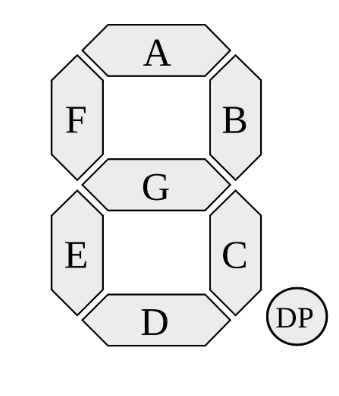
\includegraphics[width = 0.2\textwidth]{images/seven_seg_indecator.png}
    \caption{семисегментное световое табло}
    \label{fig:seven_seg_indicator}
\end{wrapfigure}

В этом задании мы составим логическую схему декодера для семисегментного индикатора. На рис. \ref{fig:seven_seg_indicator} дано изображение семисегментного
индикатора. Пользуясь таблицей истинности табл. \ref{table:logic_table}, не трудно составить
принципиальную схему дешифратора.

\begin{table}[]
\centering
\begin{tabular}{|c|cccc|ccccccc|}
\hline
\multirow{2}{*}{Цифра} & \multicolumn{4}{c|}{двоично-десятичный вход}                                     & \multicolumn{7}{c|}{семисегментный выход}                                                                                                               \\ \cline{2-12} 
                       & \multicolumn{1}{c|}{X1} & \multicolumn{1}{c|}{X2} & \multicolumn{1}{c|}{X3} & X4 & \multicolumn{1}{c|}{a} & \multicolumn{1}{c|}{b} & \multicolumn{1}{c|}{c} & \multicolumn{1}{c|}{d} & \multicolumn{1}{c|}{e} & \multicolumn{1}{c|}{f} & g \\ \hline
0                      & \multicolumn{1}{c|}{0}  & \multicolumn{1}{c|}{0}  & \multicolumn{1}{c|}{0}  & 0  & \multicolumn{1}{c|}{1} & \multicolumn{1}{c|}{1} & \multicolumn{1}{c|}{1} & \multicolumn{1}{c|}{1} & \multicolumn{1}{c|}{1} & \multicolumn{1}{c|}{1} & 0 \\ \hline
1                      & \multicolumn{1}{c|}{0}  & \multicolumn{1}{c|}{0}  & \multicolumn{1}{c|}{0}  & 1  & \multicolumn{1}{c|}{0} & \multicolumn{1}{c|}{1} & \multicolumn{1}{c|}{1} & \multicolumn{1}{c|}{0} & \multicolumn{1}{c|}{0} & \multicolumn{1}{c|}{0} & 0 \\ \hline
2                      & \multicolumn{1}{c|}{0}  & \multicolumn{1}{c|}{0}  & \multicolumn{1}{c|}{1}  & 0  & \multicolumn{1}{c|}{1} & \multicolumn{1}{c|}{1} & \multicolumn{1}{c|}{0} & \multicolumn{1}{c|}{1} & \multicolumn{1}{c|}{1} & \multicolumn{1}{c|}{0} & 1 \\ \hline
3                      & \multicolumn{1}{c|}{0}  & \multicolumn{1}{c|}{0}  & \multicolumn{1}{c|}{1}  & 1  & \multicolumn{1}{c|}{1} & \multicolumn{1}{c|}{1} & \multicolumn{1}{c|}{1} & \multicolumn{1}{c|}{1} & \multicolumn{1}{c|}{0} & \multicolumn{1}{c|}{0} & 1 \\ \hline
4                      & \multicolumn{1}{c|}{0}  & \multicolumn{1}{c|}{1}  & \multicolumn{1}{c|}{0}  & 0  & \multicolumn{1}{c|}{0} & \multicolumn{1}{c|}{1} & \multicolumn{1}{c|}{1} & \multicolumn{1}{c|}{0} & \multicolumn{1}{c|}{0} & \multicolumn{1}{c|}{1} & 1 \\ \hline
5                      & \multicolumn{1}{c|}{0}  & \multicolumn{1}{c|}{1}  & \multicolumn{1}{c|}{0}  & 1  & \multicolumn{1}{c|}{1} & \multicolumn{1}{c|}{0} & \multicolumn{1}{c|}{1} & \multicolumn{1}{c|}{1} & \multicolumn{1}{c|}{0} & \multicolumn{1}{c|}{1} & 1 \\ \hline
6                      & \multicolumn{1}{c|}{0}  & \multicolumn{1}{c|}{1}  & \multicolumn{1}{c|}{1}  & 0  & \multicolumn{1}{c|}{1} & \multicolumn{1}{c|}{0} & \multicolumn{1}{c|}{1} & \multicolumn{1}{c|}{1} & \multicolumn{1}{c|}{1} & \multicolumn{1}{c|}{1} & 1 \\ \hline
7                      & \multicolumn{1}{c|}{0}  & \multicolumn{1}{c|}{1}  & \multicolumn{1}{c|}{1}  & 1  & \multicolumn{1}{c|}{1} & \multicolumn{1}{c|}{1} & \multicolumn{1}{c|}{1} & \multicolumn{1}{c|}{0} & \multicolumn{1}{c|}{0} & \multicolumn{1}{c|}{0} & 0 \\ \hline
8                      & \multicolumn{1}{c|}{1}  & \multicolumn{1}{c|}{0}  & \multicolumn{1}{c|}{0}  & 0  & \multicolumn{1}{c|}{1} & \multicolumn{1}{c|}{1} & \multicolumn{1}{c|}{1} & \multicolumn{1}{c|}{1} & \multicolumn{1}{c|}{1} & \multicolumn{1}{c|}{1} & 1 \\ \hline
9                      & \multicolumn{1}{c|}{1}  & \multicolumn{1}{c|}{0}  & \multicolumn{1}{c|}{0}  & 1  & \multicolumn{1}{c|}{1} & \multicolumn{1}{c|}{1} & \multicolumn{1}{c|}{1} & \multicolumn{1}{c|}{1} & \multicolumn{1}{c|}{0} & \multicolumn{1}{c|}{1} & 1 \\ \hline
\end{tabular}
\caption{Таблица истиности}
\label{table:logic_table}
\end{table}

Прежде всего необходимо составить логическую функцию для каждого из выходов $a, b, \dots, g$. Для этого мы воспользуемся СДНФ.

\begin{enumerate}
    \item Выход $a$: $(X_1 \Or X_2 \Or X_3 \Or \Not{X_4}) \AND (X_1 \Or \Not{X_2} \Or X_3 \Or X_4)$
    \item Выход $b$: $(X_1 \Or \Not{X_2} \Or X_3 \Or \Not{X_4}) \AND (X_1 \Or \Not{X_2} \Or \Not{X_3} \Or X_4)$
    \item Выход $c$: $(X_1 \Or X_2 \Or \Not{X_3} \Or X_4)$
    \item Выход $d$: $(X_1 \Or X_2 \Or X_3 \Or \Not{X_4}) \AND (X_1 \Or \Not{X_2} \Or X_3 \Or X_4) \AND (X_1 \Or \Not{X_2} \Or \Not{X_3} \Or \Not{X_4})$
    \item Выход $e$: $(X_1 \Or X_2 \Or X_3 \Or \Not{X_4}) \AND (X_1 \Or X_2 \Or \Not{X_3} \Or \Not{X_4}) \AND (X_1 \Or \Not{X_2} \Or X_3 \Or X_4) \AND (X_1 \Or \Not{X_2} \Or X_3 \Or \Not{X_4}) \AND (X_1 \Or \Not{X_2} \Or \Not{X_3} \Or \Not{X_4}) \AND (\Not{X_1} \Or X_2 \Or X_3 \Or \Not{X_4})$
    \item Выход $f$: $(X_1 \Or X_2 \Or X_3 \Or \Not{X_4}) \AND (X_1 \Or X_2 \Or \Not{X_3} \Or X_4) \AND (X_1 \Or X_2 \Or \Not{X_3} \Or \Not{X_4}) \AND (X_1 \Or \Not{X_2} \Or \Not{X_3} \Or \Not{X_4})$
    \item Выход $g$: $(X_1 \Or X_2 \Or X_3 \Or X_4) \AND (X_1 \Or X_2 \Or X_3 \Or \Not{X_4}) \AND (X_1 \Or \Not{X_2} \Or \Not{X_3} \Or \Not{X_4})$
\end{enumerate}

Заметим, что в логических функциях для разных выходов некоторые логические множетели повторяются. Выпишем для удобства набор уникальных логических полиномов.

\begin{center}
    $X_1 \Or X_2 \Or X_3 \Or \Not{X_4}$ \\
    $X_1 \Or \Not{X_2} \Or X_3 \Or X_4$ \\
    $X_1 \Or \Not{X_2} \Or X_3 \Or \Not{X_4}$ \\
    $X_1 \Or \Not{X_2} \Or \Not{X_3} \Or X_4$ \\
    $X_1 \Or X_2 \Or \Not{X_3} \Or X_4$ \\
    $X_1 \Or \Not{X_2} \Or \Not{X_3} \Or \Not{X_4}$ \\
    $X_1 \Or X_2 \Or \Not{X_3} \Or \Not{X_4}$ \\
    $\Not{X_1} \Or X_2 \Or X_3 \Or \Not{X_4}$ \\
    $X_1 \Or X_2 \Or X_3 \Or X_4$ \\
\end{center}

Используя составленные логические функции и набор уникальных логических сумм нетрудно нарисовать принципиальную схему, используя базовые логические элементы рис. \ref{fig:Logic_scheme}.

%% Поскольку код логической схемы формирует файл, не
%  помещающийся в стандартные типографские размеры, 
%  схему вставим в качестве картинки
\begin{landscape}
    \begin{figure}
        \centering
        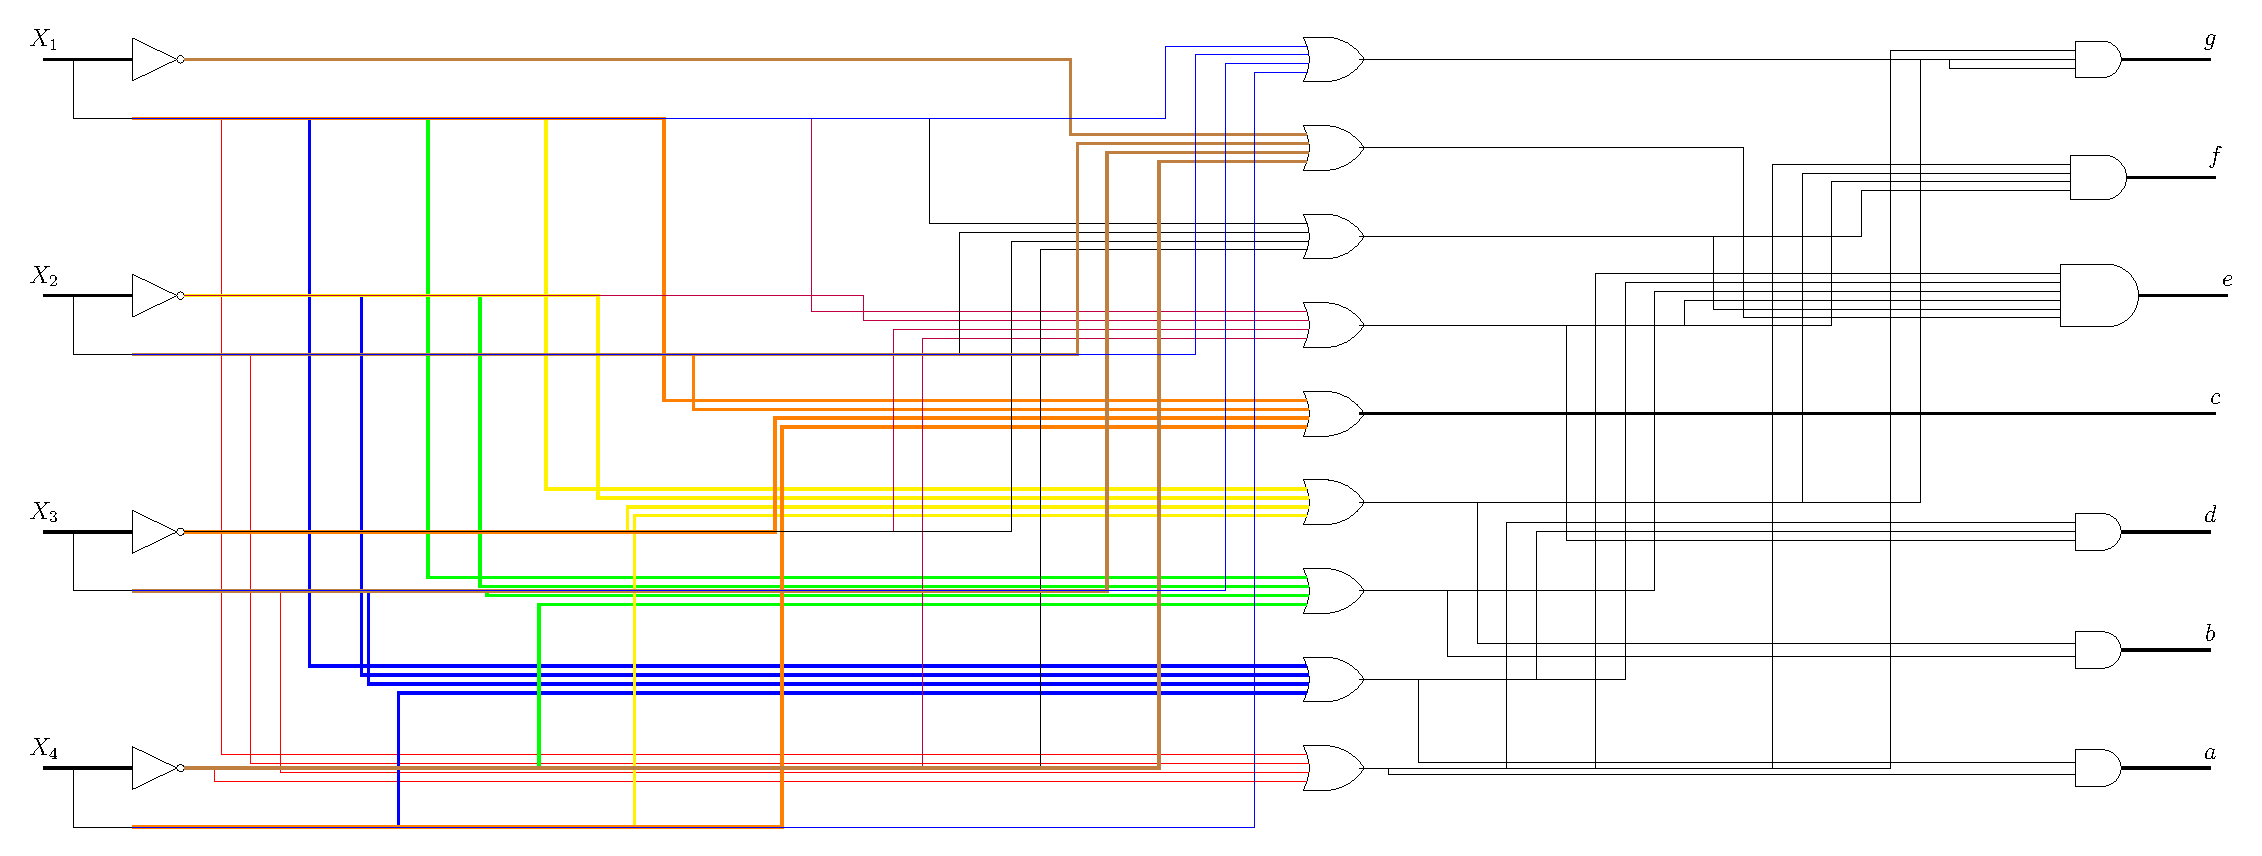
\includegraphics[scale=0.69]{images/test_logic_schems.pdf}
        \caption{Logic scheme}
        \label{fig:Logic_scheme}
    \end{figure}
\end{landscape}

\end{document}